\documentclass[border=3pt,tikz]{standalone}
\usepackage{amsmath}
\usetikzlibrary{calc}
\usetikzlibrary{arrows.meta} % for arrow size
\begin{document}
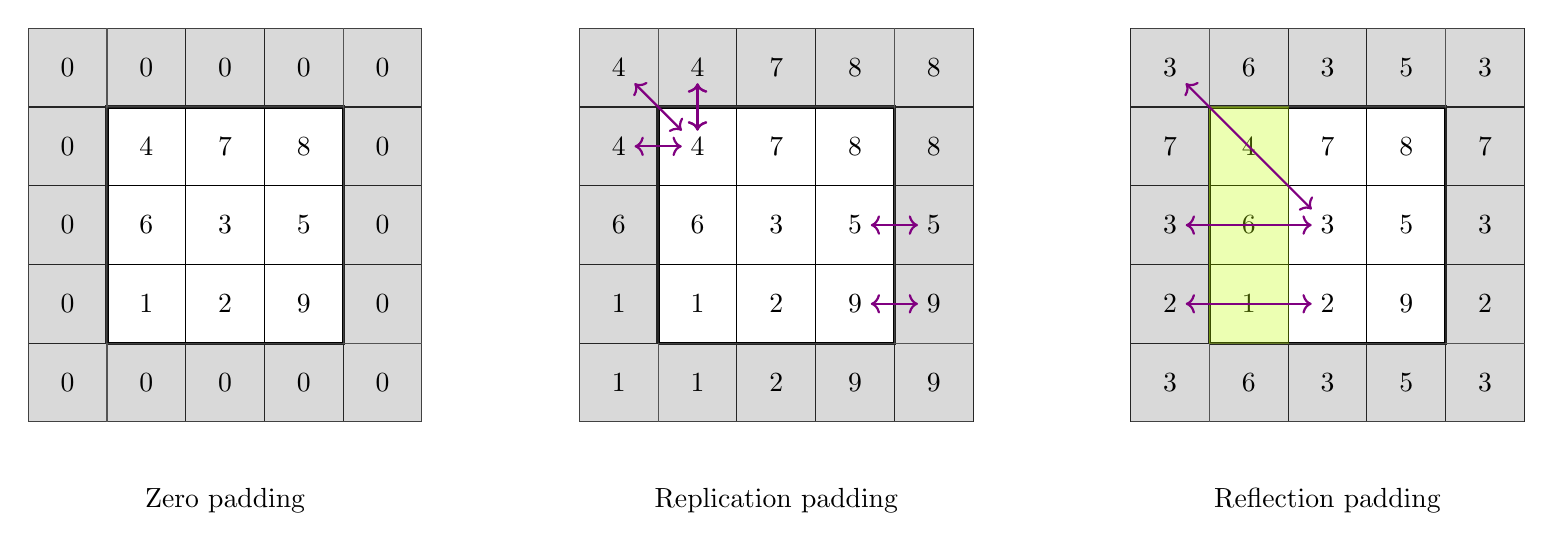
\begin{tikzpicture}[scale=1, rotate=0]
    \draw[step=1.0,black,thin] (-1,-1) grid (4,4);
    \draw[very thick] (0, 0) -- (3, 0) -- (3, 3) -- (0, 3) -- (0, 0);
    \node[] at (0.5, 0.5) {$1$};
    \node[] at (0.5, 1.5) {$6$};
    \node[] at (0.5, 2.5) {$4$};
    \node[] at (1.5, 0.5) {$2$};
    \node[] at (1.5, 1.5) {$3$};
    \node[] at (1.5, 2.5) {$7$};
    \node[] at (2.5, 0.5) {$9$};
    \node[] at (2.5, 1.5) {$5$};
    \node[] at (2.5, 2.5) {$8$};
    \filldraw [gray,opacity=0.3] (-1,-1) rectangle (0,4);
    \filldraw [gray,opacity=0.3] (0,-1) rectangle (4,0);
    \filldraw [gray,opacity=0.3] (3,0) rectangle (4,4);
    \filldraw [gray,opacity=0.3] (0,3) rectangle (3,4);

    \node[] at(-0.5, -0.5) {$0$};
    \node[] at(-0.5, 0.5) {$0$};
    \node[] at(-0.5, 1.5) {$0$};
    \node[] at(-0.5, 2.5) {$0$};
    \node[] at(-0.5, 3.5) {$0$};
    \node[] at(0.5, 3.5) {$0$};
    \node[] at(1.5, 3.5) {$0$};
    \node[] at(2.5, 3.5) {$0$};
    \node[] at(3.5, 3.5) {$0$};
    \node[] at(3.5, 2.5) {$0$};
    \node[] at(3.5, 1.5) {$0$};
    \node[] at(3.5, 0.5) {$0$};
    \node[] at(3.5, -.5) {$0$};
    \node[] at(2.5, -.5) {$0$};
    \node[] at(1.5, -.5) {$0$};
    \node[] at(0.5, -.5) {$0$};
    \node[align=center] at (1.5, -2) {Zero padding};

    \begin{scope}[xshift=7cm]
        \draw[step=1.0,black,thin] (-1,-1) grid (4,4);
        \draw[very thick] (0, 0) -- (3, 0) -- (3, 3) -- (0, 3) -- (0, 0);
        \node[] at (0.5, 0.5) {$1$};
        \node[] at (0.5, 1.5) {$6$};
        \node[] at (0.5, 2.5) {$4$};
        \node[] at (1.5, 0.5) {$2$};
        \node[] at (1.5, 1.5) {$3$};
        \node[] at (1.5, 2.5) {$7$};
        \node[] at (2.5, 0.5) {$9$};
        \node[] at (2.5, 1.5) {$5$};
        \node[] at (2.5, 2.5) {$8$};
        \filldraw [gray,opacity=0.3] (-1,-1) rectangle (0,4);
        \filldraw [gray,opacity=0.3] (0,-1) rectangle (4,0);
        \filldraw [gray,opacity=0.3] (3,0) rectangle (4,4);
        \filldraw [gray,opacity=0.3] (0,3) rectangle (3,4);
    
        \node[] at(-0.5, -0.5) {$1$};
        \node[] at(-0.5, 0.5) {$1$};
        \node[] at(-0.5, 1.5) {$6$};
        \node[] at(-0.5, 2.5) {$4$};
        \node[] at(-0.5, 3.5) {$4$};
        \node[] at(0.5, 3.5) {$4$};
        \node[] at(1.5, 3.5) {$7$};
        \node[] at(2.5, 3.5) {$8$};
        \node[] at(3.5, 3.5) {$8$};
        \node[] at(3.5, 2.5) {$8$};
        \node[] at(3.5, 1.5) {$5$};
        \node[] at(3.5, 0.5) {$9$};
        \node[] at(3.5, -.5) {$9$};
        \node[] at(2.5, -.5) {$9$};
        \node[] at(1.5, -.5) {$2$};
        \node[] at(0.5, -.5) {$1$};
        \node[align=center] at (1.5, -2) {Replication padding};
        \draw[violet, thick, <->] (-0.3, 2.5) -- (0.3, 2.5);
        \draw[violet, thick, <->] (-0.3, 3.3) -- (0.3, 2.7);
        \draw[violet, thick, <->] (0.5, 3.3) -- (0.5, 2.7);
        \draw[violet, thick, <->] (0.5, 3.3) -- (0.5, 2.7);
        \draw[violet, thick, <->] (2.7, 1.5) -- (3.3, 1.5);
        \draw[violet, thick, <->] (2.7, 0.5) -- (3.3, 0.5);
    \end{scope}


    \begin{scope}[xshift=14cm]
        \draw[step=1.0,black,thin] (-1,-1) grid (4,4);
        \draw[very thick] (0, 0) -- (3, 0) -- (3, 3) -- (0, 3) -- (0, 0);
        \node[] at (0.5, 0.5) {$1$};
        \node[] at (0.5, 1.5) {$6$};
        \node[] at (0.5, 2.5) {$4$};
        \node[] at (1.5, 0.5) {$2$};
        \node[] at (1.5, 1.5) {$3$};
        \node[] at (1.5, 2.5) {$7$};
        \node[] at (2.5, 0.5) {$9$};
        \node[] at (2.5, 1.5) {$5$};
        \node[] at (2.5, 2.5) {$8$};
        \filldraw [gray,opacity=0.3] (-1,-1) rectangle (0,4);
        \filldraw [gray,opacity=0.3] (0,-1) rectangle (4,0);
        \filldraw [gray,opacity=0.3] (3,0) rectangle (4,4);
        \filldraw [gray,opacity=0.3] (0,3) rectangle (3,4);
    
        \node[] at(-0.5, -0.5) {$3$};
        \node[] at(-0.5, 0.5) {$2$};
        \node[] at(-0.5, 1.5) {$3$};
        \node[] at(-0.5, 2.5) {$7$};
        \node[] at(-0.5, 3.5) {$3$};
        \node[] at(0.5, 3.5) {$6$};
        \node[] at(1.5, 3.5) {$3$};
        \node[] at(2.5, 3.5) {$5$};
        \node[] at(3.5, 3.5) {$3$};
        \node[] at(3.5, 2.5) {$7$};
        \node[] at(3.5, 1.5) {$3$};
        \node[] at(3.5, 0.5) {$2$};
        \node[] at(3.5, -.5) {$3$};
        \node[] at(2.5, -.5) {$5$};
        \node[] at(1.5, -.5) {$3$};
        \node[] at(0.5, -.5) {$6$};
        \node[align=center] at (1.5, -2) {Reflection padding};

        \filldraw [lime,opacity=0.3] (0,0) rectangle (1,3);
        \draw[violet, thick, <->] (-0.3, 0.5) -- (1.3, 0.5);
        \draw[violet, thick, <->] (-0.3, 1.5) -- (1.3, 1.5);
        \draw[violet, thick, <->] (-0.3, 3.3) -- (1.3, 1.7);
    
    \end{scope}
  \end{tikzpicture}
\end{document}